\documentclass{article}
\usepackage{booktabs}
\usepackage{caption}
\usepackage[margin=1in]{geometry}
\usepackage{graphicx}
\usepackage{float}
\usepackage{array}
\usepackage{siunitx}
\sisetup{scientific-notation=true}

\begin{document}
\title{Rocket Stage Optimization Report}
\author{Generated by Payload Optimization Script}
\maketitle

\section{Problem Definition}
\subsection{Input Parameters}
\begin{table}[H]
\centering
\caption{Global Parameters}
\begin{tabular}{lc}
\toprule
Parameter & Value \\
\midrule
G0 & 9.81 \\
\bottomrule
\end{tabular}
\end{table}

\begin{table}[H]
\centering
\caption{Stage Parameters}
\begin{tabular}{ccc}
\toprule
Stage & ISP & $\epsilon$ \\
\midrule
1 & 300.0 & 0.060 \\
2 & 348.0 & 0.040 \\
\bottomrule
\end{tabular}
\end{table}

\section{Optimization Results}
\subsection{Performance Comparison}
\begin{table}[H]
\centering
\caption{Solver Performance}
\begin{tabular}{lccc}
\toprule
Method & Payload Fraction & Execution Time (s) & Convergence \\
\midrule
SLSQP & 0.032 & 0.00 & Yes \\
DIFFERENTIAL_EVOLUTION & 0.036 & 0.37 & Yes \\
BASIN-HOPPING & 0.032 & 0.57 & Yes \\
GA-ADAPTIVE & 0.036 & 0.15 & Yes \\
PSO & 0.036 & 0.88 & Yes \\
\bottomrule
\end{tabular}
\end{table}

\subsection{Stage-wise Results}

\subsubsection{SLSQP}
\begin{table}[H]
\centering
\caption{SLSQP Stage Results}
\begin{tabular}{cccc}
\toprule
Stage & $\Delta V$ (m/s) & Mass Ratio & Contribution (\%) \\
\midrule
1 & 4650.0 & 0.146 & 50.0 \\
2 & 4650.0 & 0.216 & 50.0 \\
\bottomrule
\end{tabular}
\end{table}

\subsubsection{DIFFERENTIAL_EVOLUTION}
\begin{table}[H]
\centering
\caption{DIFFERENTIAL_EVOLUTION Stage Results}
\begin{tabular}{cccc}
\toprule
Stage & $\Delta V$ (m/s) & Mass Ratio & Contribution (\%) \\
\midrule
1 & 2772.9 & 0.330 & 29.8 \\
2 & 6527.1 & 0.108 & 70.2 \\
\bottomrule
\end{tabular}
\end{table}

\subsubsection{BASIN-HOPPING}
\begin{table}[H]
\centering
\caption{BASIN-HOPPING Stage Results}
\begin{tabular}{cccc}
\toprule
Stage & $\Delta V$ (m/s) & Mass Ratio & Contribution (\%) \\
\midrule
1 & 4649.7 & 0.146 & 50.0 \\
2 & 4650.3 & 0.216 & 50.0 \\
\bottomrule
\end{tabular}
\end{table}

\subsubsection{GA-ADAPTIVE}
\begin{table}[H]
\centering
\caption{GA-ADAPTIVE Stage Results}
\begin{tabular}{cccc}
\toprule
Stage & $\Delta V$ (m/s) & Mass Ratio & Contribution (\%) \\
\midrule
1 & 2773.0 & 0.330 & 29.8 \\
2 & 6527.0 & 0.108 & 70.2 \\
\bottomrule
\end{tabular}
\end{table}

\subsubsection{PSO}
\begin{table}[H]
\centering
\caption{PSO Stage Results}
\begin{tabular}{cccc}
\toprule
Stage & $\Delta V$ (m/s) & Mass Ratio & Contribution (\%) \\
\midrule
1 & 2773.0 & 0.330 & 29.8 \\
2 & 6527.0 & 0.108 & 70.2 \\
\bottomrule
\end{tabular}
\end{table}

\section{Visualizations}
\begin{figure}[H]
\centering
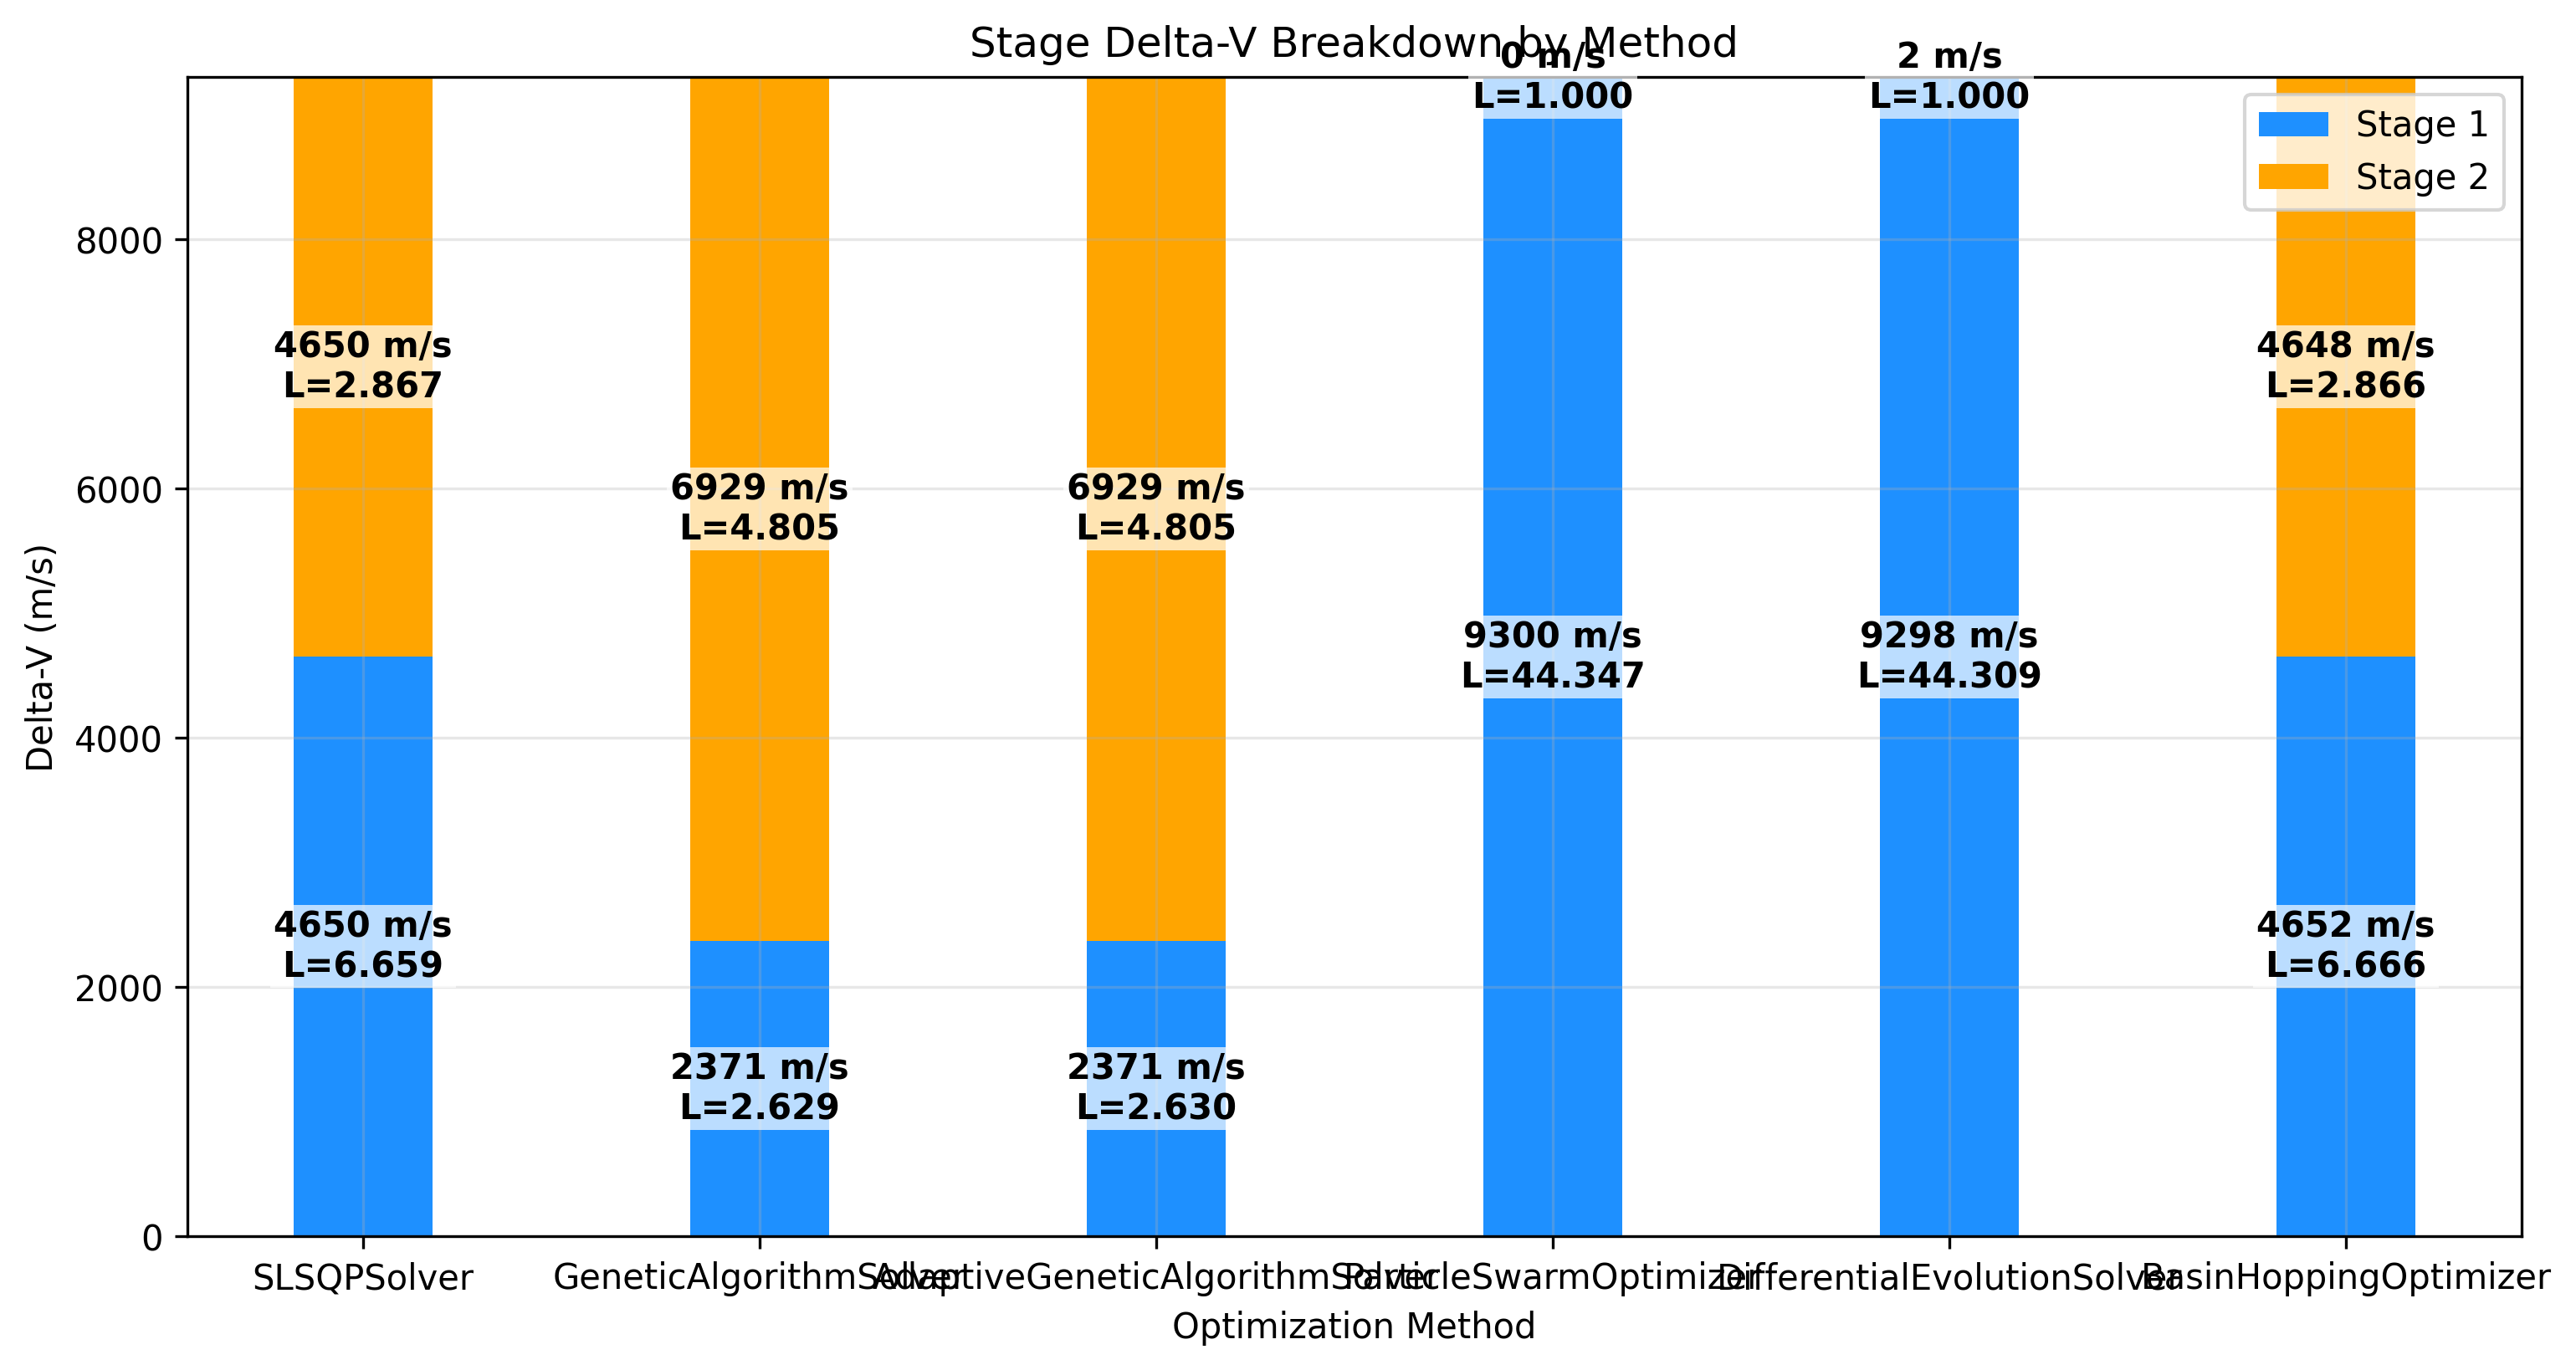
\includegraphics[width=\textwidth]{dv_breakdown.png}
\caption{$\Delta V$ Distribution Across Stages}
\end{figure}

\begin{figure}[H]
\centering
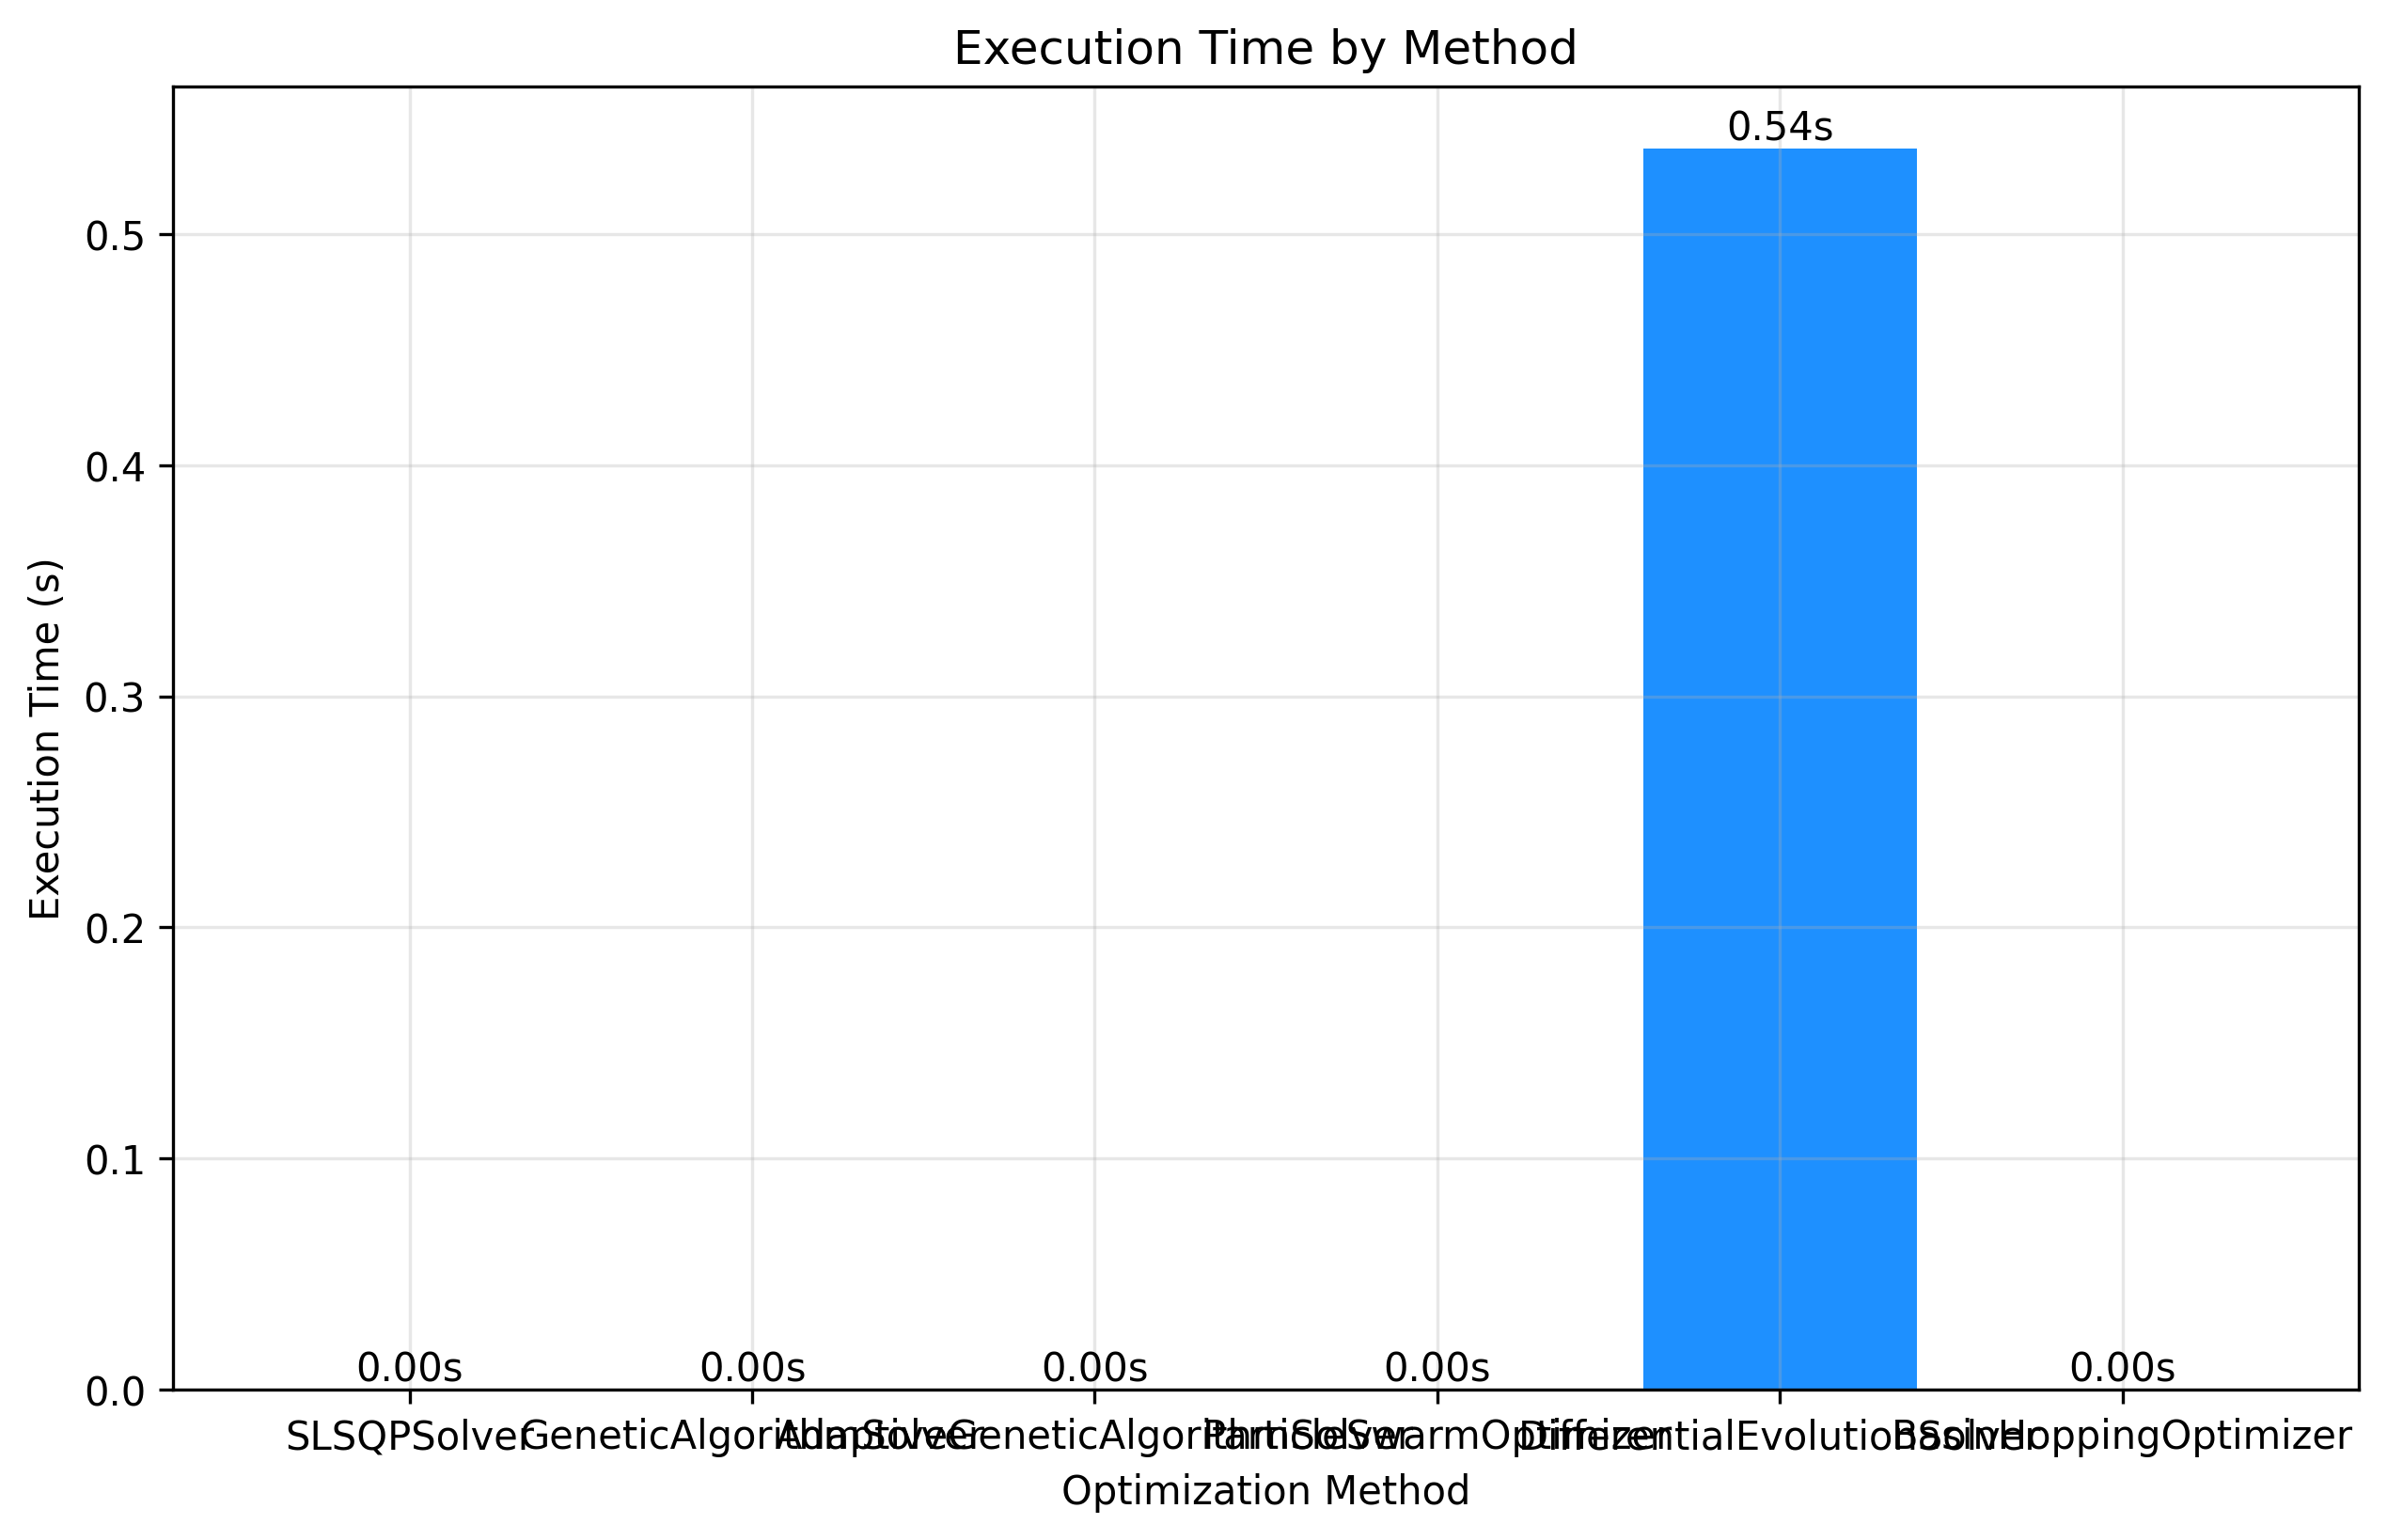
\includegraphics[width=\textwidth]{execution_time.png}
\caption{Solver Execution Time Comparison}
\end{figure}

\begin{figure}[H]
\centering
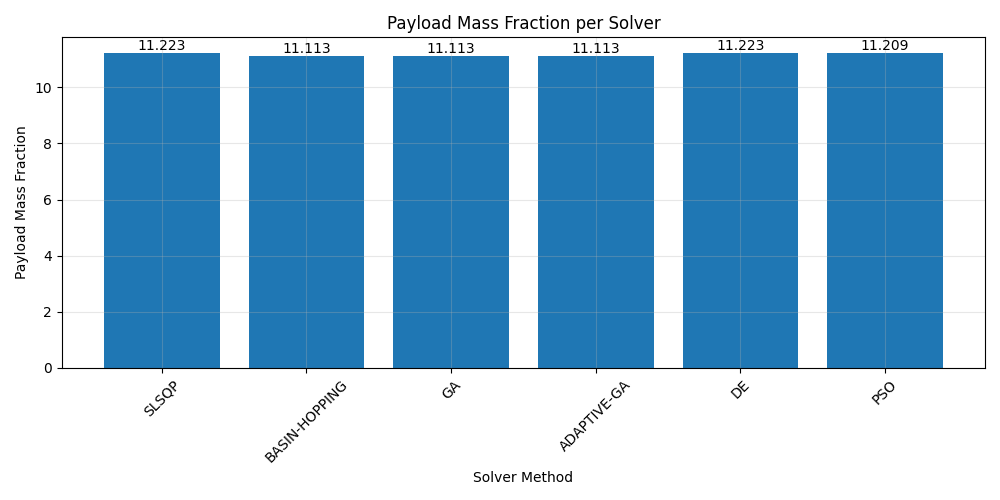
\includegraphics[width=\textwidth]{payload_fraction.png}
\caption{Payload Fraction Comparison}
\end{figure}

\end{document}
